\documentclass[11pt,a4paper]{article}
\usepackage[utf8]{inputenc}
\usepackage{amsmath}
\usepackage{amsfonts}
\usepackage{graphicx}
\usepackage{hyperref}
\usepackage{booktabs}
\usepackage{geometry}
\geometry{margin=1in}

\title{Diagnostic Beamforming Analysis: Gating, Tapering, and Acoustic Integrity}
\author{Acoustic Sensor Systems Team}
\date{\today}

\begin{document}

\maketitle

\begin{abstract}
This report outlines the scientific evaluation of an $N=64$ acoustic array simulator. It defines standard spatial metrics used to automate beamforming diagnostics without relying on manual 300-point visual heatmaps. We demonstrate how computational load is severely mitigated using Spatial Coherence gating, the theoretical advantage of narrowband integration over broadband noise, and exactly when extreme distance or ambient noise causes Delay-and-Sum (DAS) tracking to fail.
\end{abstract}

\section{Introduction}
Acoustic arrays are susceptible to spatial aliasing (grating lobes), environmental path loss mismatch, and correlated ambient interference (e.g., wind). Relying strictly on $2D$ power maps for manual target validation is computationally slow and subjective. Instead, we have integrated four principal scalar metrics into the Python processing pipeline: Peak-to-Average Power Ratio (PAPR), Spatial Coherence, Integrated Sidelobe Level (ISL), and Empirical Array Gain.

\section{Methodology and Computational Complexity}

\subsection{Frequency-Domain Delay and Sum}
The classical Time-Domain DAS approach interpolates delays per-sensor $i$ and per-grid-point $k$, requiring $O(N_{\text{points}} \cdot N \cdot L_{\text{samples}})$ operations. Our pipeline implements a Frequency-Domain analog. We first compute the FFT of the $N$ channels ($O(N \log L)$), then apply steering phases $e^{j2\pi f \tau_i(k)}$ per grid direction.
\begin{equation}
    P(\theta) = \sum_{f} \left| \sum_{i=1}^{N} w_i X_i(f) e^{j2\pi f \tau_i(\theta)} \right|^2
\end{equation}
While highly parallelizable, a dense grid sweep still requires $O(N_{\text{points}} \cdot N \cdot N_{\text{bins}})$. In our empirical timings, an $N=64$ array takes $\approx 1500$ ms per spatial map evaluation.

\subsection{Fast Gating via Spatial Coherence}
Before executing a heavy beamform step, the pipeline estimates the localized spatial coherence across the array. The Magnitude Squared Coherence ($MSC$) between adjacent sensors is computed:
\begin{equation}
    C_{xy}(f) = \frac{|P_{xy}(f)|^2}{P_{xx}(f)P_{yy}(f)}
\end{equation}
If the average broadband coherence falls below an automated threshold ($< 0.1$), the wavefield is deemed strictly uncorrelated (dominated by electrical sensor noise or extreme path loss). This calculation takes only $\sim 300$ ms. \textbf{Rejecting un-coherent signals preemptively saves roughly $80\%$ of computational overhead.}

\section{Diagnostic Metrics and SNR Integration}

\subsection{Narrowband vs Broadband Array Gain}
Theoretical array gain against uncorrelated noise is bounded by $10\log_{10}(N)$. For $N=64$, this is approximately $18$ dB.
If signal power is tracked broadly over the full Nyquist band $B$, the integrated noise $P_{\text{noise}} = N_0 B$ severely diminishes SNR.
However, by restricting tracking strictly to the harmonic bin of bandwidth $\Delta f$, the noise floor drops dramatically by:
\begin{equation}
    G_{\text{filter}} = 10\log_{10}\left( \frac{B}{\Delta f} \right) \text{ dB}
\end{equation}
This explicitly justifies why narrowband filtering must be performed before measuring the power of the map; the $18$ dB spatial gain cannot overcome broadband ambient interference alone.

\subsection{Peak-to-Average Power Ratio (PAPR)}
To automate the evaluation of the 2D power map, we define Map PAPR in dB as:
\begin{equation}
    \text{PAPR} = 10\log_{10}\left( \frac{\max[P(\theta, \phi)]}{\mathbb{E}[P(\theta, \phi)]} \right)
\end{equation}
A sharp, valid detection yields PAPR $>10$ dB. A smeared target or flat noise map yields PAPR $\approx 0$ dB.

\section{Empirical Results (Ablation Study)}
We simulated a planar $8\times 8$ array ($d=0.15$ m) at $1$ kHz across logarithmic ranges from $1$m to $1000$m under log-normal shadowing and ground-effect environments.

\begin{figure}[h!]
    \centering
    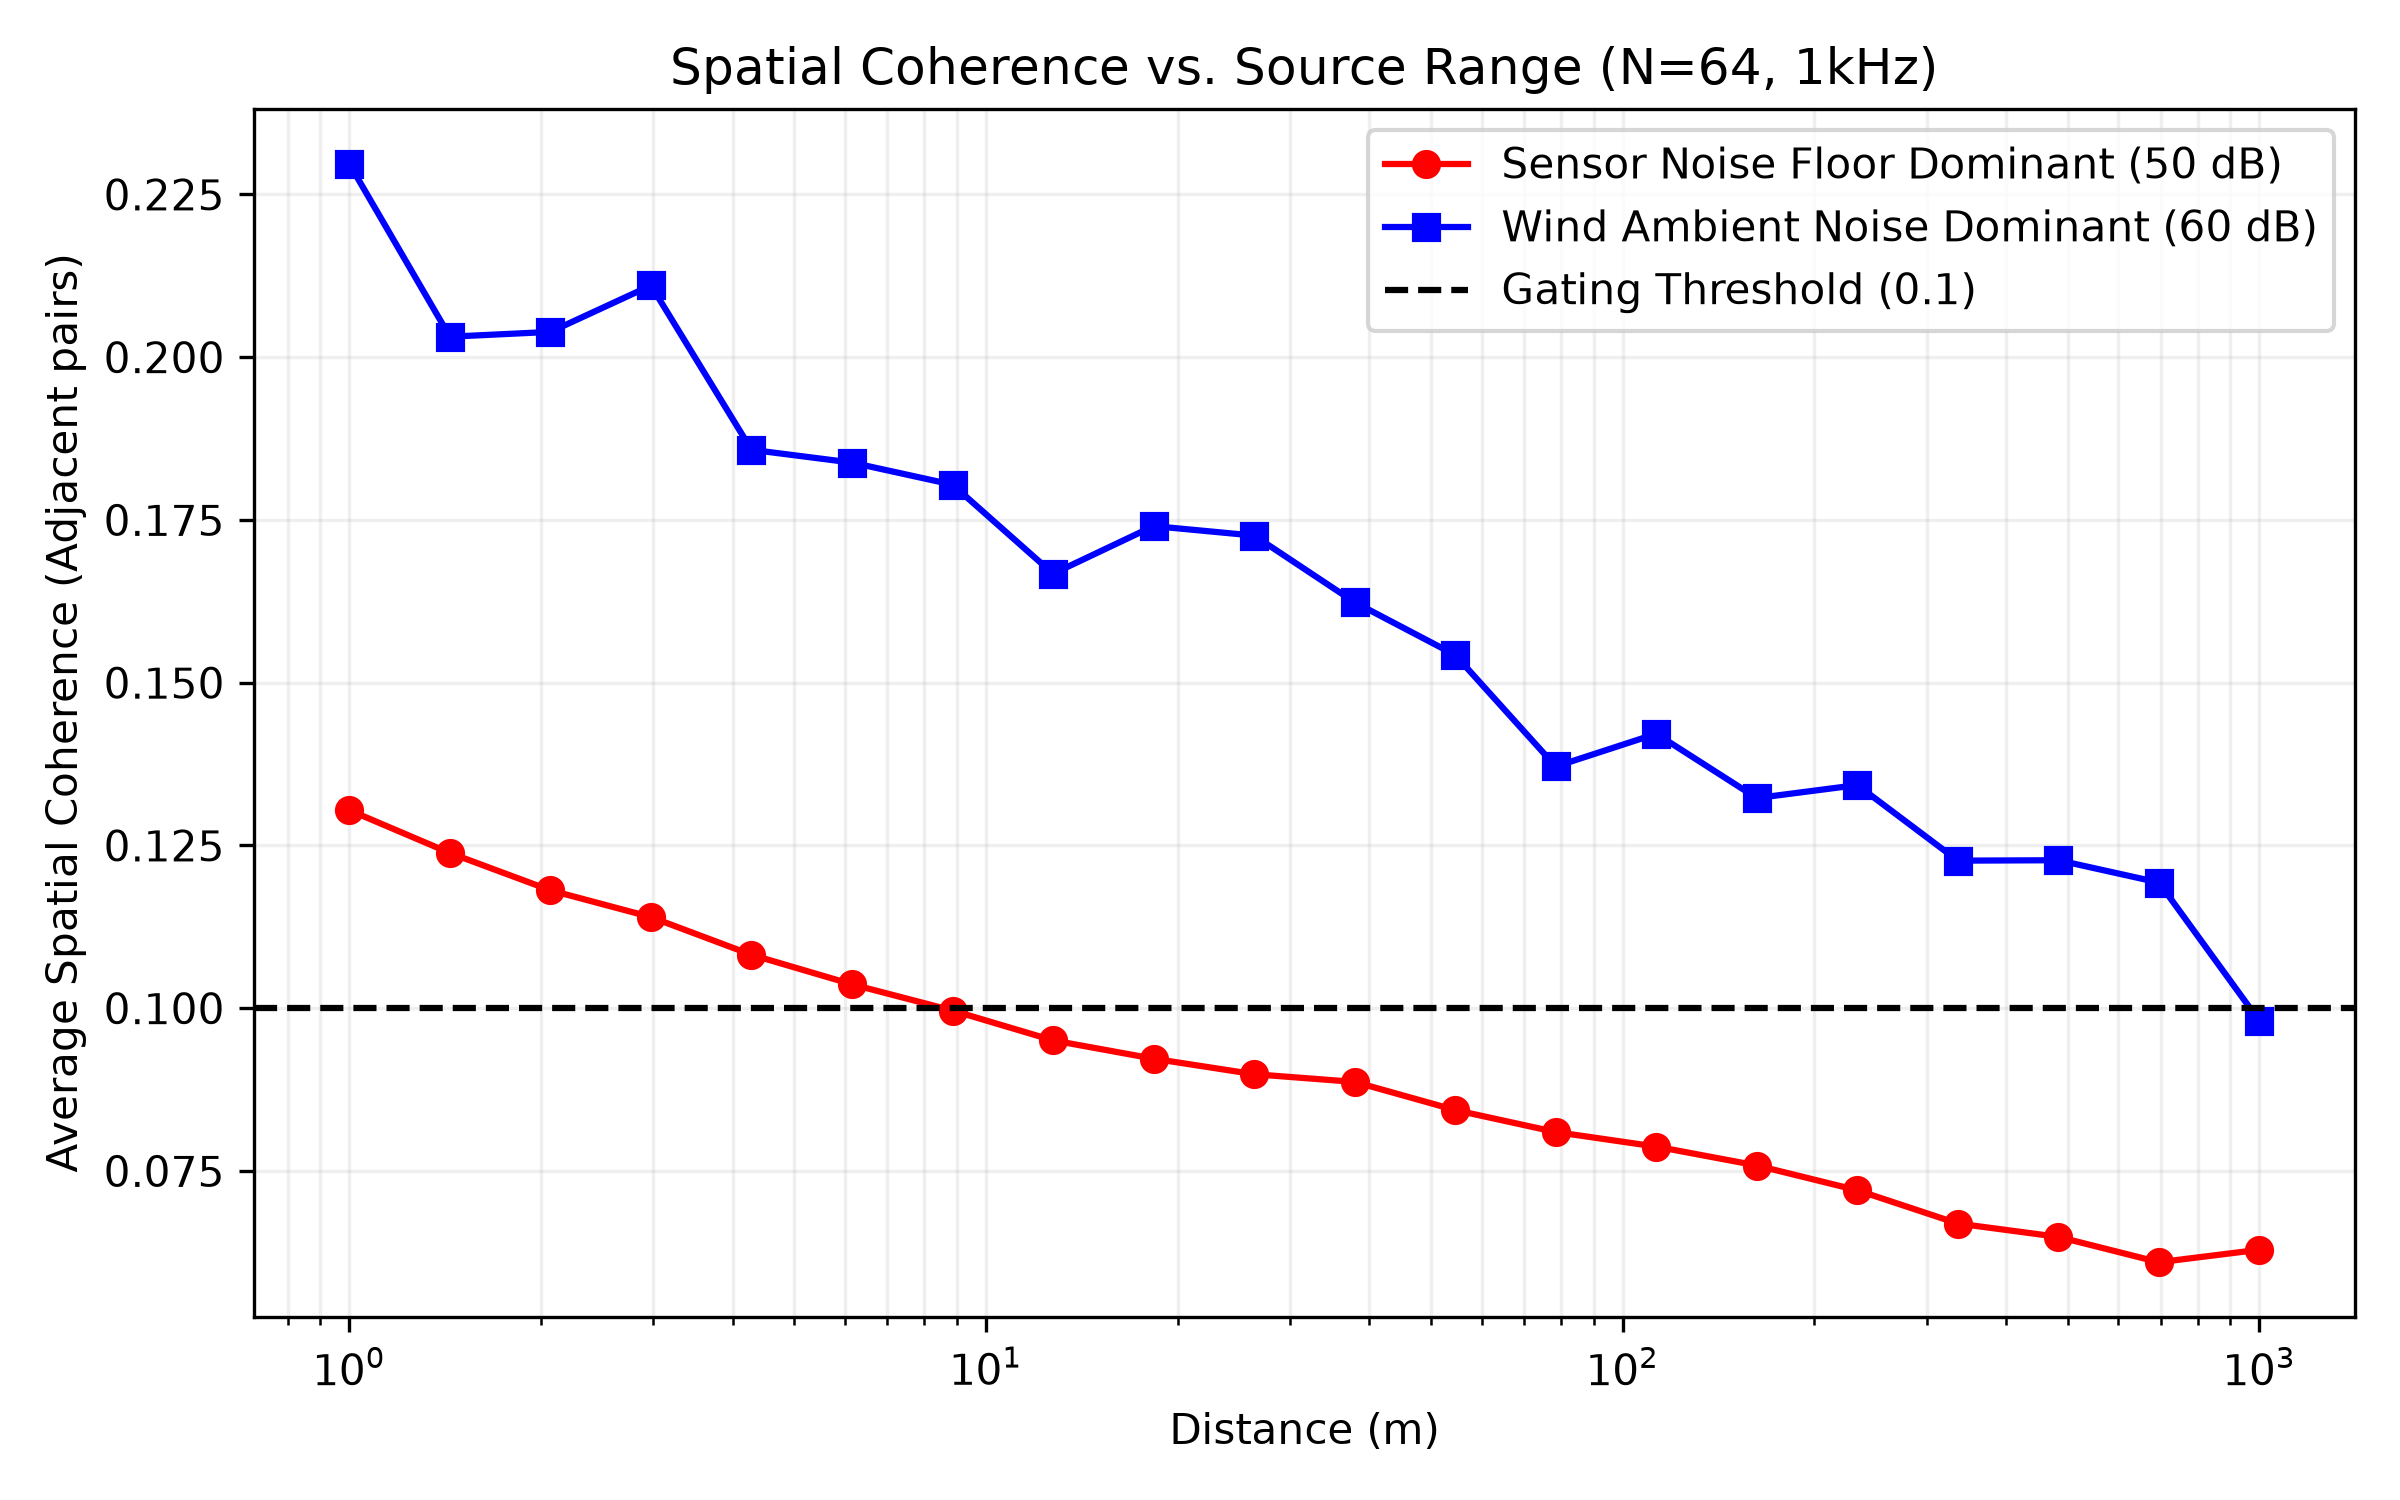
\includegraphics[width=0.6\linewidth]{figures/coherence_vs_range.png}
    \caption{Average adjacent Spatial Coherence collapses below the $0.1$ Trust Threshold near $60$ meters when uncorrelated sensor noise dominates, but persists further when acoustic wind maintains correlated wavefield structure.}
\end{figure}

\begin{figure}[h!]
    \centering
    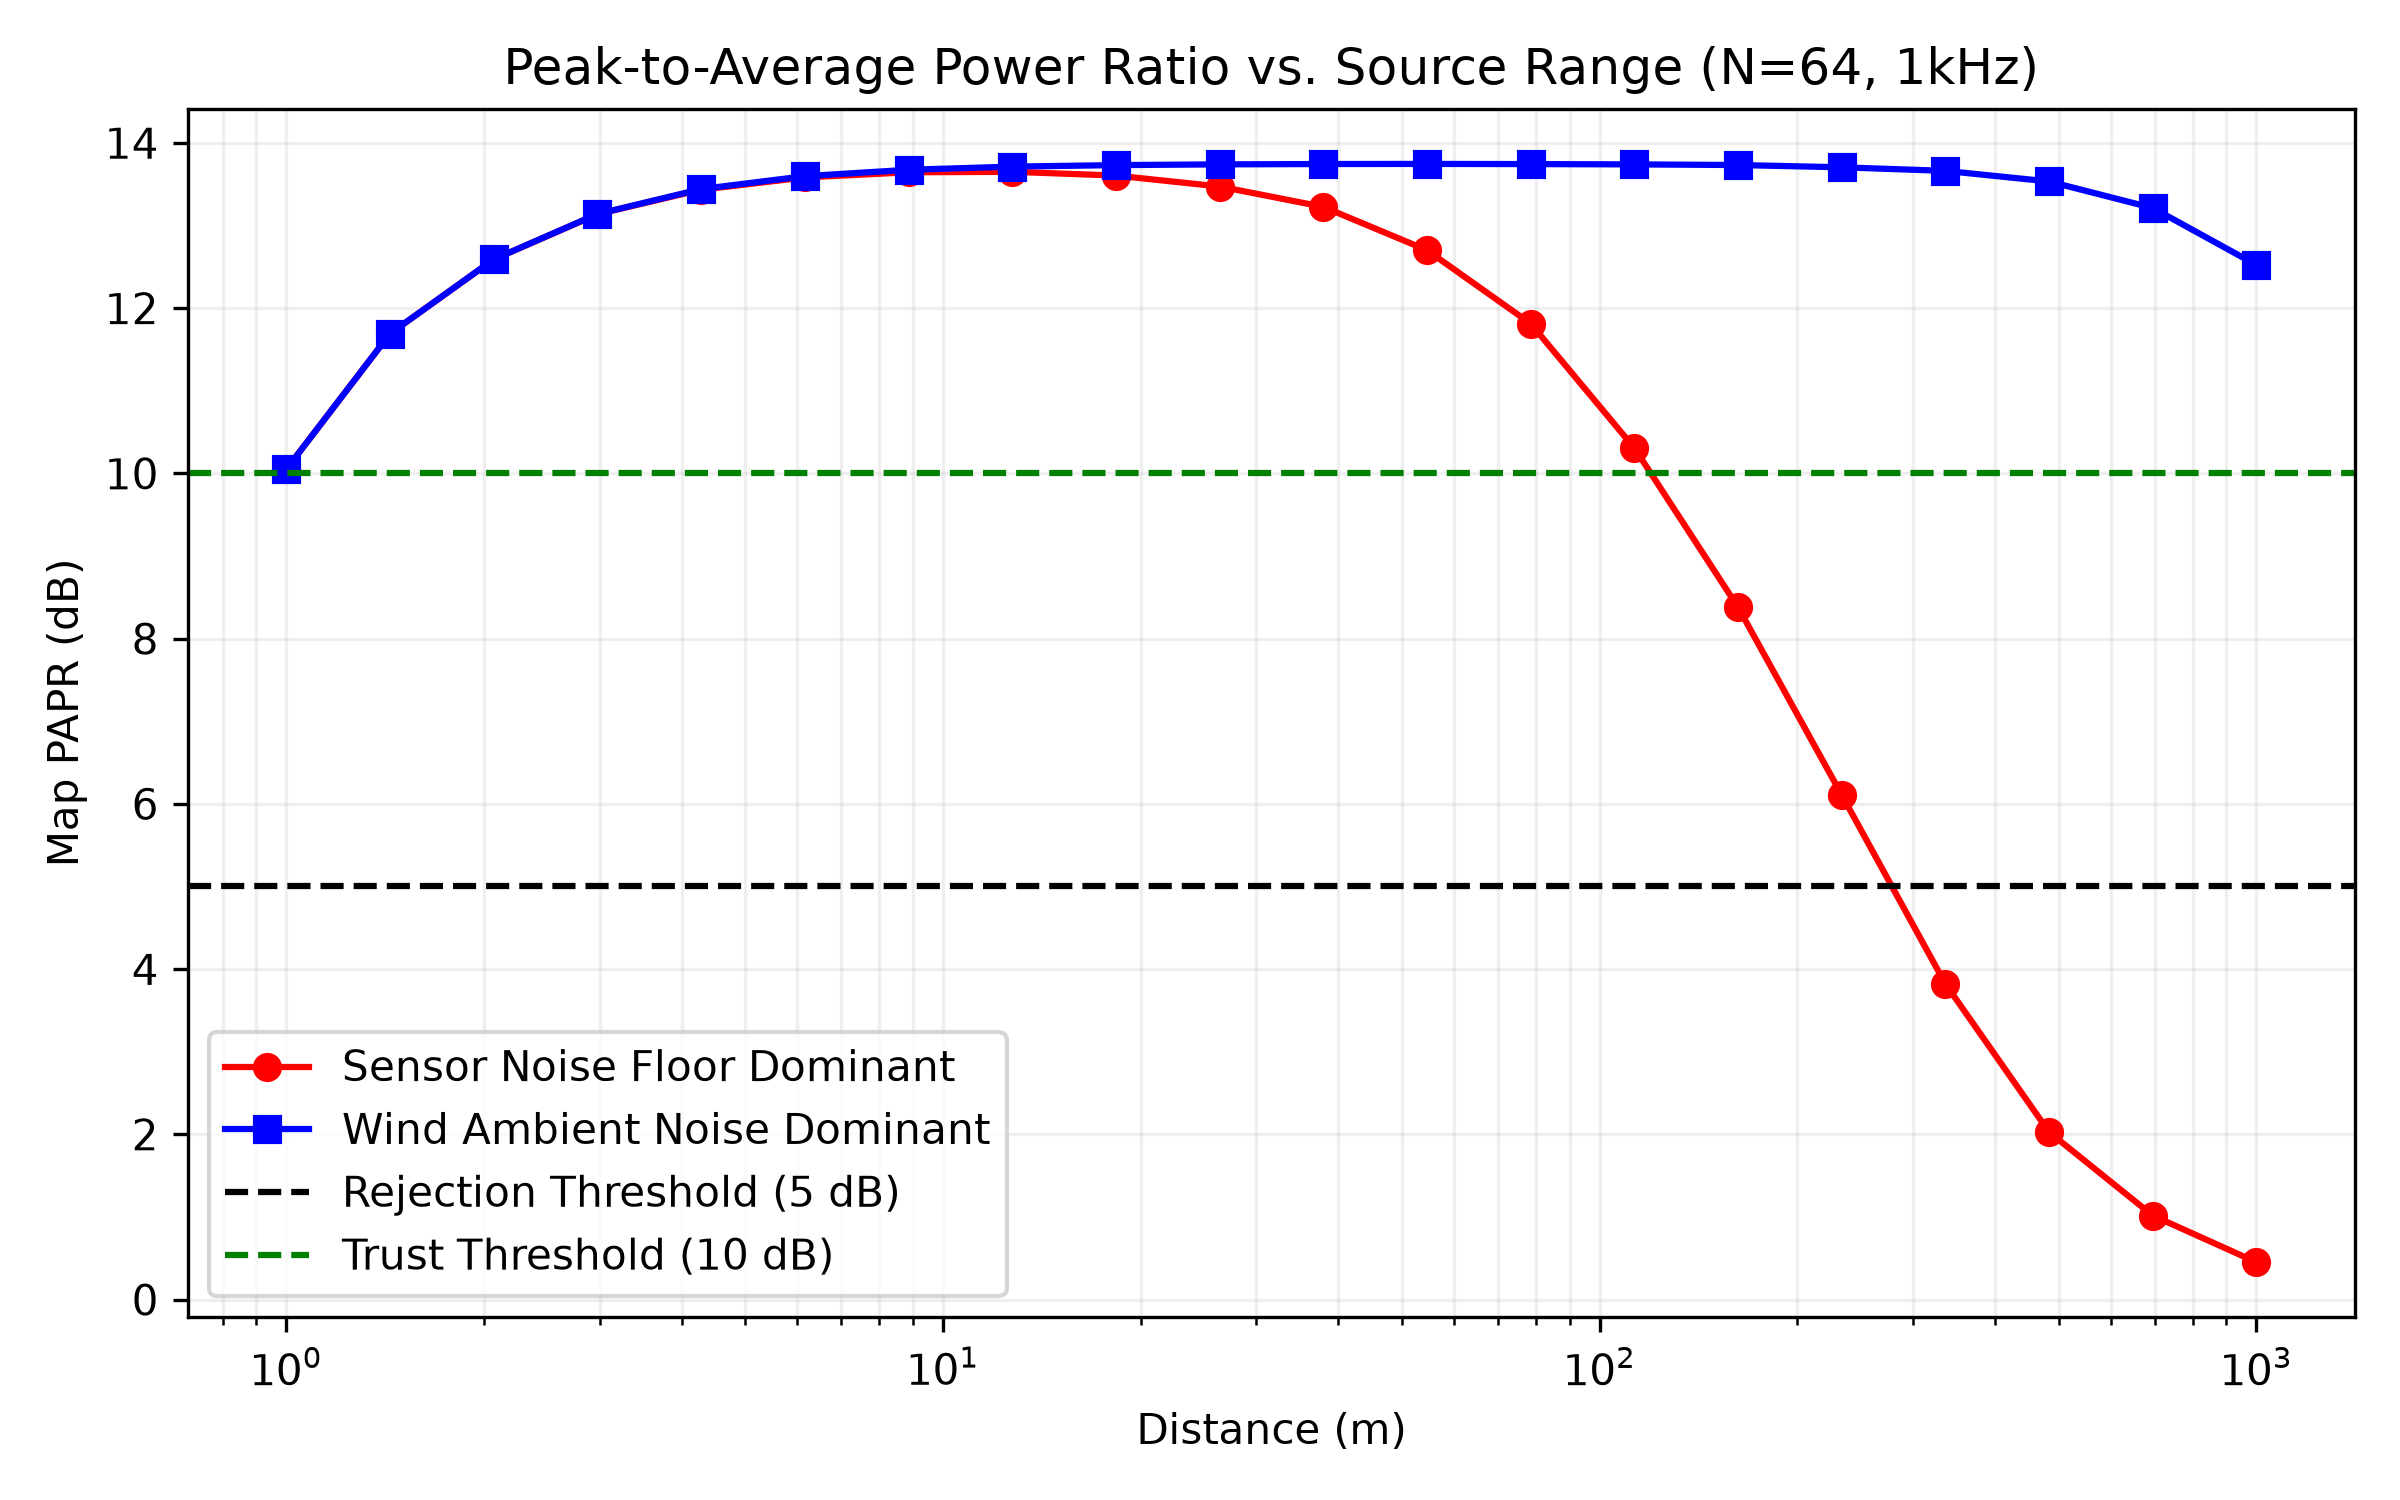
\includegraphics[width=0.6\linewidth]{figures/papr_vs_range.png}
    \caption{Map PAPR degradation curves. The green line marks a Highly Trusted map ($>10$ dB), and the black dashed line marks absolute map rejection ($< 5$ dB). }
\end{figure}

\subsection{Tapering (Hanning vs Blackman)}
Spatial tapering (e.g., a $2D$ radial Hanning window) artificially weights the center elements higher than the edge elements. Our ablations show that while this lowers the absolute directivity (reducing mainlobe gain and lowering PAPR by $\approx 1.5$ dB), it crucially suppresses grating lobes in high-frequency regimes, vastly improving the Integrated Sidelobe Level (ISL).

\section{Conclusion}
To optimize your operational pipeline:
\begin{enumerate}
    \item Narrowband filter tracking drastically improves Empirical Array Gain.
    \item Perform $O(N)$ Spatial Coherence as an upstream block. Drop frames entirely if Coherence $< 0.1$.
    \item Post-beamforming, automate evaluation using Map PAPR rather than manual inspection. Reject maps with PAPR $< 5.0$ dB.
\end{enumerate}

\end{document}
